%
% Layout retirado de http://www.di.uminho.pt/~prh/curplc09.html#notas
%
\documentclass{report}
%encoding
%--------------------------------------
\usepackage[utf8]{inputenc}
\usepackage[T1]{fontenc}
%--------------------------------------

%Portuguese-specific commands
%--------------------------------------
\usepackage[portuguese]{babel}
%--------------------------------------

%Hyphenation rules
%--------------------------------------
\usepackage{hyphenat}
\hyphenation{mate-mática recu-perar}
%--------------------------------------

\usepackage{url}
\usepackage{enumerate}
\usepackage{graphicx}

%\usepackage{alltt}
%\usepackage{fancyvrb}
\usepackage{listings}
%LISTING - GENERAL
\lstset{
    basicstyle=\small,
    numbers=left,
    numberstyle=\tiny,
    numbersep=5pt,
    breaklines=true,
    frame=tB,
    mathescape=true,
    escapeinside={(*@}{@*)}
}
%
%\lstset{ %
%   language=Java,                          % choose the language of the code
%   basicstyle=\ttfamily\footnotesize,      % the size of the fonts that are used for the code
%   keywordstyle=\bfseries,                 % set the keyword style
%   %numbers=left,                          % where to put the line-numbers
%   numberstyle=\scriptsize,                % the size of the fonts that are used for the line-numbers
%   stepnumber=2,                           % the step between two line-numbers. If it's 1 each line
%                                           % will be numbered
%   numbersep=5pt,                          % how far the line-numbers are from the code
%   backgroundcolor=\color{white},          % choose the background color. You must add \usepackage{color}
%   showspaces=false,                       % show spaces adding particular underscores
%   showstringspaces=false,                 % underline spaces within strings
%   showtabs=false,                         % show tabs within strings adding particular underscores
%   frame=none,                             % adds a frame around the code
%   %abovecaptionskip=-.8em,
%   %belowcaptionskip=.7em,
%   tabsize=2,                              % sets default tabsize to 2 spaces
%   captionpos=b,                           % sets the caption-position to bottom
%   breaklines=true,                        % sets automatic line breaking
%   breakatwhitespace=false,                % sets if automatic breaks should only happen at whitespace
%   title=\lstname,                         % show the filename of files included with \lstinputlisting;
%                                           % also try caption instead of title
%   escapeinside={\%*}{*)},                 % if you want to add a comment within your code
%   morekeywords={*,...}                    % if you want to add more keywords to the set
%}

\usepackage{xspace}

\parindent=0pt
\parskip=2pt

\setlength{\oddsidemargin}{-1cm}
\setlength{\textwidth}{18cm}
\setlength{\headsep}{-1cm}
\setlength{\textheight}{23cm}

\def\darius{\textsf{Darius}\xspace}
\def\antlr{\texttt{AnTLR}\xspace}
\def\pl{\emph{Processamento de Linguagens}\xspace}

\def\titulo#1{\section{#1}}
\def\super#1{{\em Supervisor: #1}\\ }
\def\area#1{{\em \'{A}rea: #1}\\[0.2cm]}
\def\resumo{\underline{Resumo}:\\ }


%%%%\input{LPgeneralDefintions}

\title{Processamento de Linguagens (3º ano do MiEI)\\ \textbf{Trabalho Prático 1 - Parte B}\\ Flex - Processador de Inglês corrente}
\author{Gustavo Andrez\\ (A27748) \and Rogério Moreira\\ (A74634) \and Samuel Ferreira\\ (A76507) }
\date{\today}

\begin{document}

\maketitle

\begin{abstract}

O presente trabalho tem como objetivo aumentar a experiência no uso do ambiente Linux, aumentar capacidade de escrever Expressões Regulares (ER) e, a partir destas,  desenvolver Processadores de Linguagens Regulares.
A ferramenta de processamento de texto utilizada é o C Flex que, por sua vez, também utiliza o GCC. Todos os objetivos inicialmente propostos foram cumpridos.

\end{abstract}

\tableofcontents

\chapter{Introdu\c{c}\~ao} \label{intro}

\section*{Introdu\c{c}\~ao} \

A diversidade e quantidade de informação nos dias de hoje é cada vez maior e mais dispersa, está em todo o lado em grandes quantidades, a todo o momento. Posto isto, torna-se ainda mais necessária uma linguagem de programação como o C Flex, que permite filtrar, de maneira facilitada, a informação essencial num ficheiro em que os dados estejam dispersos e ainda tratar essa informação. O trabalho apresentado na unidade curricular de Processamento de Linguagens tem como objetivo usar esta ferramenta para filtrar um conjunto de dados fornecidos, extraindo desses dados informação relevante.

\section*{Sele\c{c}\~ao de enunciados} \

O tema escolhido pelo grupo foi "Processador de Inglês corrente" cuja descrição apresentamos em seguida.
\\“Neste projeto pretende-se que leiam um texto corrente em inglês que faça uso das habituais contrações do tipo I'm, I'll, We're, can't, it's e:
\begin{itemize}
\item[a)] reproduza o texto de entrada na saída expandindo todas as contrações que encontrar.
\item[b)] gere em HTML uma lista ordenada de todos os verbos (no infinitivo não flexionado) que encontrar no texto, recordando que essa forma verbal em inglês precedida pela palavra to, sendo a mesma palavra retirada se o dito verbo for antecedido por can, could, shall, should, will, would, may, might. Considere também a forma interrogativa em que o verbo no infinitivo é precedido por do/does ou did.”
\end{itemize}

\section*{Objetivos}
Para o desenvolvimento deste trabalho foram definidos os seguintes objetivos:
\\
\begin{itemize}
\item Conseguir expandir corretamente um número elevado de contrações presentes num texto em língua inglesa;
\item Identificar, com uma taxa de correção elevada, os verbos no infinitivo constantes num texto em língua inglesa.
\end{itemize}
\newpage
\section*{Estrutura do Relatório} \

Inicialmente vai ser explicado o problema, as características dos dados fornecidos e os padrões de frase por nós encontrados e que levaram à resolução dos problemas inicialmente propostos.\\
Numa segunda fase apresentamos a codificação em Flex da solução desenvolvida mostrando as estruturas de dados e ações semânticas, bem como alternativas e decisões tomadas face aos problemas de implementação.\\
Em seguida mostramos exemplo de um input e output e, posteriormente, é feita uma análise de resultado onde se explicam a realização de alguns testes para caracterizar a solução encontrada.\\
Em apêndice a este relatório está também todo o código desenvolvido.

\section*{Características dos Dados, Padr\~oes de Frase e Decisões}

O programa a desenvolver tem por propósito receber textos em língua inglesa. Neste idioma é comum a utilização de contrações. Assim, quando estas forem detectadas far-se-á a respectiva expansão. Para isto foi necessário investigar sobre as contrações possíveis e decidir acerca de quais os casos a serem cobertos. De uma forma geral, decidiu-se cobrir todos os casos mais comuns de contrações tanto específicos (p.ex. gonna) como gerais (p.ex. we’ll).\\
Relativamente à recolha de verbos no infinitivo, para os localizar, considerou-se que se encontram precedidos por palavras características (p.ex. to e may). No entanto, nos casos em que a frase se encontra na forma interrogativa, entre as palavras atrás referidas e o verbo, usualmente é encontrado um pronome. Assim, assumiu-se que é um verbo no infinito a palavra que é precedida de um pronome e uma das palavras atrás referidas e seguido por um ponto de interrogação.

\chapter{Implementação e Ações Semânticas} \label{ae}
\section{Expansão de contrações}
Em seguida são discriminadas as expressões irregulares responsáveis por expandir as contrações detectadas bem como alguns exemplos abrangidos pelas mesmas.
\\
\begin{verbatim}
[gG]onna[\.\?\!\;,\ \n\t] {printf("%coing to%c",yytext[0],yytext[strlen(yytext)-1]);}
\end{verbatim}
Gonna -> Going to      e 	gonna -> going to
\\
\begin{verbatim}
[wW]anna[\.\?\!\;,\ \n\t]     { printf("%cant to%c",yytext[0],yytext[strlen(yytext)-1]); }
\end{verbatim}
Wanna -> Want to    e     wanna -> want to
\\
\begin{verbatim}
[cC]an't[\.\?\!\;,\ \n\t]     { printf("%cannot%c",yytext[0],yytext[strlen(yytext)-1]); }
\end{verbatim}
Can't -> Cannot    e     can't -> cannot
\\
\begin{verbatim}
[wW]on't[\.\?\!\;,\ \n\t]   {printf("%cill not%c",yytext[0],yytext[strlen(yytext)-1]);}
\end{verbatim}
Won't -> Will not    e     won't -> will not
\\
\begin{verbatim}
I\ ain't[\.\?\!\;,\ \n\t]    { printf("I am not%c",yytext[strlen(yytext)-1]); }
\end{verbatim}
I ain't -> I am not
\\
\begin{verbatim}
([hH]e|[sS]he|[iI]t)\ ain't[\.\?\!\;,\ \n\t]
{ printf("%s is not%c",strtok(yytext,""),yytext[strlen(yytext)-1]);}
\end{verbatim}
He / She / It ain't -> He / She / It is not
e
he / she / it ain't -> he / she / it is not
\\
\begin{verbatim}
([yY]ou|[tT]hey|[wW]e)\ ain't[\.\?\!\;,\ \n\t]
{ printf("%s are not%c",strtok(yytext," "),yytext[strlen(yytext)-1]);}
\end{verbatim}
You / They / We ain't -> You / They / We are not
e
you / they / we ain't -> you / they / we are not
\\
\begin{verbatim}
[tT]hat\ ain't[\.\?\!\;,\ \n\t]
{ printf("%chat is not%c",yytext[0],yytext[strlen(yytext)-1]);}
\end{verbatim}
That ain't -> That is not
e
that ain't -> that is not
\\
\begin{verbatim}
[tT]his\ ain't[\.\?\!\;,\ \n\t]  { printf("%chis is not%c",yytext[0],yytext[strlen(yytext)-1]);}
\end{verbatim}
This ain't -> This is not
e
this ain't -> this is not

\\
\begin{verbatim}
\'[cC]ause[\.\?\!\;,\ \n\t]  { printf("%cecause%c", yytext[1]-1,yytext[strlen(yytext)-1]); }
\end{verbatim}
'Cause -> Because
       e
'cause -> because

\\
Neste caso Yytext[1]-1 coloca o caratere “b” ou “B” consoante o “c” identificado seja minúsculo ou maiúsculo, ou seja, subtrai uma unidade ao código ASCII do “c” ou “C” resultando em “b” ou “B”.
\\
\begin{verbatim}
'm[\.\?\!\;,\ \n\t]    { printf(" am%c",yytext[strlen(yytext)-1]); }
\end{verbatim}
I’m -> I am
\\
\begin{verbatim}
're[\.\?\!\;,\ \n\t]    { printf(" are%c",yytext[strlen(yytext)-1]); }
\end{verbatim}
're -> are
\\
Por exemplo:
You're -> You are    e     what're -> what are

\\
\begin{verbatim}
n't[\.\?\!\;,\ \n\t]    { printf(" not%c",yytext[strlen(yytext)-1]); }
\end{verbatim}
n't -> not
Por exemplo:
Didn't -> Did not    e     weren't -> were not
\\
\begin{verbatim}
'll[\.\?\!\;,\ \n\t] { printf(" will%c",yytext[strlen(yytext)-1]); }
\end{verbatim}
'll -> will
\\
Por exemplo:
What'll -> What will    e     she'll -> she will
\\
Neste caso assumiu-se que a contração “'ll” corresponderá na grande maioria dos casos à extensão “will” e não “shall”. Por isto considerou-se que quando aparece esta contração será desdobrada em “will”.

\\
\begin{verbatim}
've[\.\?\!\;,\ \n\t]    { printf(" have%c",yytext[strlen(yytext)-1]); }
\end{verbatim}
've -> have
\\
Por exemplo:
You've -> You have    e     might've -> might have

\\
\begin{verbatim}
'd[\.\?\!\;,\ \n\t]    { printf(" would%c",yytext[strlen(yytext)-1]); }
\end{verbatim}
'd -> would
\\
Por exemplo:
I'd -> I would    e     how'd -> how would

\\
\begin{verbatim}
's[\.\?\!\;,\ \n\t]    { printf(" [is/has]%c",yytext[strlen(yytext)-1]); }
\end{verbatim}
's -> is ou has
\\
Por exemplo:
She's -> She [is/has]   e  that's -> that [is/has]

Neste caso considerámos que a contração “‘s” poderá corresponder a “is” ou “has” com probabilidades próximas. Assim optou-se por não assumir uma das opções mas sim apresentar ambas deixando ao critério do utilizador a sua interpretação, utilizando uma ou outra consoante o contexto da frase.
\\
\\
\section{Recolha de verbos}

Para a recolha de verbos no infinitivo foi seguido o seguinte algoritmo, em que se mostram as correspondentes expressões regulares:
\\
\begin{enumerate}
\item Cada vez que é  detectada uma das seguintes palavras  (com a primeiro caractere maiúsculo ou minúsculo), o estado é alterado de INITIAL para VERBO.
\\
\{to, can, can't, could, shall, should, will, would, may, might, did, didn't\}

\begin{verbatim}
[^a-zA-Z]+(?i:(to|can('t)?|could|shall|should|will|would|may|might|did(n't)))\ + { ECHO; BEGIN VERBO; }
\end{verbatim}


\item Caso a palavra sucessora da identificada no passo 1 seja uma das seguintes palavras (com a primeiro caractere maiúsculo ou minúsculo), o estado é alterado de VERBO para INTERROG (passo 2.1).

\\
\{i, me, my, myself, mine, you, your, yours, yourself, he, him, himself, his, she, her, hers, herself, it, its, we, us, our, ours, ourselves, the, they, them, themselves, a, this, that\}

\begin{verbatim}
<VERBO>(?i:(i|me|my(self)?|mine|you(r|rs|rself)?|he|him(self)?|his|she|her(s|self)?|it(s)?|we|us|
our(s|selves)?|the(y)|them(selves)?|a|th(is|at)))[\.\?\!\;\',\:\ \n\t]  { ECHO ; BEGIN INTERROG;}
\end{verbatim}

\begin{enumerate}
\item Nesta altura assumimos que a frase presente está na interrogativa e que a palavra seguinte corresponderá a um verbo caso seja a última ou a penúltima antes do sinal de ponto de interrogação. Nesse caso a palavra será um verbo e é armazenada. Por fim o estado é alterado de INTERROG para INITIAL.

\begin{verbatim}
INTERROG>[a-z]+(\ [a-z]+)?\? {
    int i=0;
    yytext[strlen(yytext)-1]='\0';
    char * aux=strtok(yytext," ");
    aux=strtok(aux,"?");
    while(i<countVerbos){
        if(strcmp(verbos[i],aux)==0)
            break;
        i++;
    }
    if(i==countVerbos)
        verbos[countVerbos++]=strdup(aux);
    ECHO;
    BEGIN INITIAL;
\end{verbatim}
\end{enumerate}

\item Nesta altura sabemos que depois das palavras explicitadas no passo 1 não está um pronome. Assim, assumimos que é um verbo este é armazenado. Por fim o estado é alterado de VERBO para INITIAL.

\begin{verbatim}
<VERBO>[a-z]+ {
    int i=0;
    while(i<countVerbos){
        if(strcmp(verbos[i],yytext)==0)
            break;
        i++;
    }
    if(i==countVerbos)
        verbos[countVerbos++]=strdup(yytext);
    ECHO;
    BEGIN INITIAL;
\end{verbatim}

\item Caso não haja correspondência no passo 3, ou seja, não é imediatamente identificada uma palavra, o estado é alterado de VERBO para INITIAL.

\begin{verbatim}
<VERBO>.|\n                    { ECHO ; BEGIN INITIAL ; }
\end{verbatim}

\end{enumerate}
\section{Apresentação do Output}
Para tratamento dos dados de input e respectiva apresentação da informação tratada foi desenvolvida a seguinte main:

\begin{verbatim}
int main(){
    yylex();
    int i=0;printf("\n\n");
    FILE *fp;
    fp= fopen("verbos.html", "w");
    qsort (verbos, countVerbos, sizeof (const char *), compare);
    fprintf(fp,"<html><body><h1>verbos:%d</h1><ul>\n",countVerbos);
    for(i=0;i<countVerbos;i++)
        fprintf(fp,"<li>to %s</li>\n",verbos[i]);
    fprintf(fp,"</ul></body></html>");
    fclose(fp);
    return 1;
}
\end{verbatim}

O texto de entrada é varrido pelo yylex() sendo apresentado no ecrã com as expansões das contrações e preenchido o array com os verbos identificados (sem repetições). Por fim, os verbos constantes do array são exportados para um ficheiro HTML (verbos.html) como uma lista ordenada alfabeticamente sendo apresentados numa página HTML bem como a contagem do número de verbos diferentes recolhidos.
\chapter{Apresentação de Resultados}
Em seguida apresentamos um pequeno exemplo de input por forma a demonstrar as funcionalidades do programa desenvolvido.
\\
\\
\section{Input - Exemplo}
\begin{verbatim}
   It's my life
   It's now or never
   I ain't gonna live forever
   I just want to live while I'm alive
   (It's my life)
   My heart is like an open highway
   Like Frankie said
   I did it my way
   I just wanna live while I'm alive
   It's my life
\end{verbatim}
\\
\section{Output - Expansão de contrações}
\begin{verbatim}
   It [is/has] my life
   It [is/has] now or never
   I am not going to live forever
   I just want to live while I am alive
   (It [is/has] my life)
   My heart is like an open highway
   Like Frankie said
   I did it my way
   I just want to live while I am alive
   It [is/has] my life
\end{verbatim}
\newpage
\section{Output - Recolha de verbos}
\begin{center}
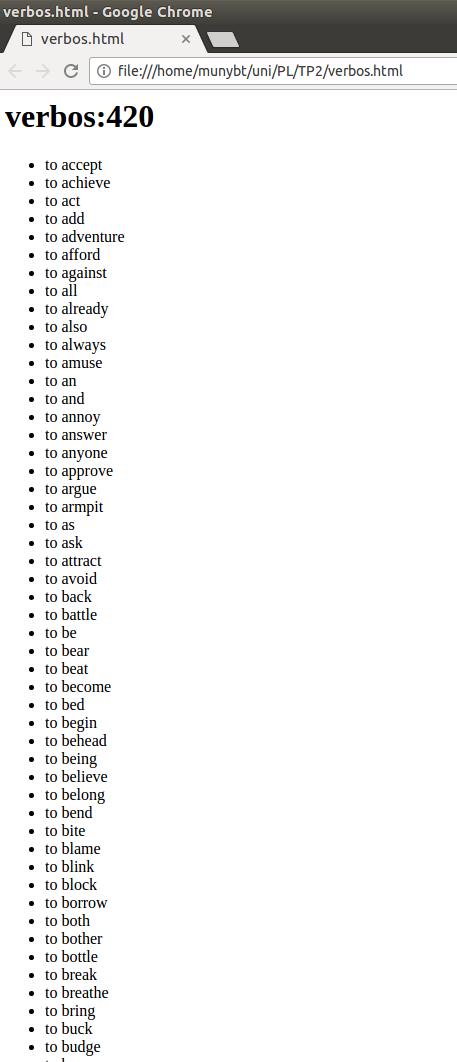
\includegraphics[scale=0.5]{print}
\end{center}
\chapter{Análise de Resultados}
Perante os resultados obtidos procedemos a uma análise onde em seguida se sintetizam alguns comentários relativos à expansão de contrações e à recolhas de verbos no infinitivo.
\\
\\
\section{Expansão de contrações}
\\
\begin{itemize}
      \item Casos em que não há dúvida na expansão é logo substituído
      \item Casos em que existe mais do que uma expansão possível e em que a probabilidade de ser uma das expansões muito elevada, utilizamos essa opção (especificamente o caso de ‘ll corresponder a will)
      \item Casos em que existe mais do que uma expansão possível, oferecemos as várias possibilidades de expansão ao utilizador que depois se encarregará de optar pela mais adequada para o  caso em questão

\end{itemize}
\\
\section{Recolha de verbos}
\\
\begin{itemize}
      \item Fez-se a recolha dos os verbos no infinitivo
      \item Testou-se com três livros: Harry Potter and the Sorcerer's Stone, The Sonnet e Eragon.
      \item Compilou-se uma lista de verbos em inglês (6057 verbos) e fez-se comparação linha a linha dos verbos recolhidos com esta lista
      \item Fizeram-se teste nos vários livros abarcando ou não as frases na interrogativa.
      \item Procedeu-se a uma aprimoração de resultados

\end{itemize}
\\
Obtivemos os seguintes resultados para o livro Eragon:
\\
\\
Total & Certos & Errados & Sucesso \\
873   & 713    & 160     & 81,67
\\
Resultados obtidos sem a deteção dos verbos no infinitivo nas frases interrogativas.
\\
\\
Total & Certos & Errados & Sucesso \\
876   & 715    & 161     & 81,62
\\
Resultados obtidos com a deteção dos verbos no infinitivo nas frases interrogativas, o verbo tem que ser obrigatoriamente a última palavra da frase.
\newpage
Total & Certos & Errados & Sucesso \\
876   & 714    & 162     & 81,50
\\
Resultados obtidos com a deteção dos verbos no infinitivo nas frases interrogativas mas em que o verbo poderá ser a última ou penúltima palavra da frases.
\\
\\
Tendo em conta os resultados obtidos e visto que, a taxa de sucesso e idêntica nos três casos optámos por dar privilégio ao número de verbos obtidos, tendo sido incluído na versão final o passo INTERROG.

\chapter{Conclusão} \label{concl}
Atendendo aos resultados obtidos, consideramos que todos os objectivos foram atingidos com sucesso.
Consideramos que o programa desenvolvido pode ser usado como ferramenta de tratamento de texto em diversos contextos.
\\
Como trabalho futuro sugerimos a inclusão de mais alguns casos de contrações e a automatização da comparação dos verbos recolhidos com uma lista de verbos de modo a eliminar os casos não válidos.

\appendix
\chapter{Código FLEX}

Lista-se a seguir o código desenvolvido.
\\
\begin{verbatim}
   %option noyywrap
   %x VERBO INTERROG
   %{
   	#include "string.h"
   	#include <stdlib.h>
   	#define MAX 3000
   	char * verbos[MAX];
   	int countVerbos=0;
   	static int compare (const void * a, const void * b){
       	return strcmp (*(const char **) a, *(const char **) b);
   	}
   %}
   %%
   [^a-zA-Z]+(?i:(to|can('t)?|could|shall|should|will|would|may|might|did(n't)))\ +  { ECHO; BEGIN VERBO; }
   <VERBO>(?i:(i|me|my(self)?|mine|you(r|rs|rself)?|he|him(self)?|his|she
   |her(s|self)?|it(s)?|we|us|our(s|selves)?|the(y)|them(selves)?|a|th(is|at)))[\.\?\!\;\',\:\ \n\t]
   { ECHO ; BEGIN INTERROG;}
   <VERBO>[a-z]+ {
   	int i=0;
   	while(i<countVerbos){
       	if(strcmp(verbos[i],yytext)==0)
           	break;
       	i++;
   	}
   	if(i==countVerbos)
       	verbos[countVerbos++]=strdup(yytext);
   	ECHO;
   	BEGIN INITIAL;
   }
   <VERBO>.|\n                	{ ECHO ; BEGIN INITIAL ; }
   <INTERROG>[a-z]+(\ [a-z]+)?\? {
   	int i=0;
   	yytext[strlen(yytext)-1]='\0';
   	char * aux=strtok(yytext," ");
   	aux=strtok(aux,"?");
   	while(i<countVerbos){
       	if(strcmp(verbos[i],aux)==0)
           	break;
       	i++;
   	}
   	if(i==countVerbos)
       	verbos[countVerbos++]=strdup(aux);
   	ECHO;
   	BEGIN INITIAL;
   }
   <INTERROG>.|\n                	{ ECHO ; BEGIN INITIAL ; }
   [gG]onna[\.\?\!\;,\ \n\t] { printf("%coing to%c",yytext[0],yytext[strlen(yytext)-1]); }
   [wW]anna[\.\?\!\;,\ \n\t] { printf("%cant to%c",yytext[0],yytext[strlen(yytext)-1]); }
   [cC]an't[\.\?\!\;,\ \n\t] { printf("%cannot%c",yytext[0],yytext[strlen(yytext)-1]); }
   [wW]on't[\.\?\!\;,\ \n\t] { printf("%cill not%c",yytext[0],yytext[strlen(yytext)-1]); }
   I\ ain't[\.\?\!\;,\ \n\t] { printf("I am not%c",yytext[strlen(yytext)-1]); }
   ([hH]e|[sS]he|[iI]t)\ ain't[\.\?\!\;,\ \n\t]
   v{ printf("%s is not%c",strtok(yytext," "),yytext[strlen(yytext)-1]);}
   ([yY]ou|[tT]hey|[wW]e)\ ain't[\.\?\!\;,\ \n\t]
   { printf("%s are not%c",strtok(yytext," "),yytext[strlen(yytext)-1]);}
   [tT]hat\ ain't[\.\?\!\;,\ \n\t]       	{ printf("%chat is not%c",yytext[0],yytext[strlen(yytext)-1]); }
   [tT]his\ ain't[\.\?\!\;,\ \n\t]       	{ printf("%chis is not%c",yytext[0],yytext[strlen(yytext)-1]); }
   \'[cC]ause[\.\?\!\;,\ \n\t]              	{ printf("%cecause%c", yytext[1]-1,yytext[strlen(yytext)-1]); }
   'm[\.\?\!\;,\ \n\t]                      	{ printf(" am%c",yytext[strlen(yytext)-1]); }
   're[\.\?\!\;,\ \n\t]                     	{ printf(" are%c",yytext[strlen(yytext)-1]); }
   n't[\.\?\!\;,\ \n\t]                     	{ printf(" not%c",yytext[strlen(yytext)-1]); }
   'll[\.\?\!\;,\ \n\t]                     	{ printf(" will%c",yytext[strlen(yytext)-1]); }
   've[\.\?\!\;,\ \n\t]                     	{ printf(" have%c",yytext[strlen(yytext)-1]); }
   'd[\.\?\!\;,\ \n\t]                      	{ printf(" would%c",yytext[strlen(yytext)-1]); }
   's[\.\?\!\;,\ \n\t]                      	{ printf(" [is/has]%c",yytext[strlen(yytext)-1]); }
   %%
   int main(){
   	yylex();
   	int i=0;printf("\n\n");
   	FILE *fp;
   	fp= fopen("verbos.html", "w");
   	qsort (verbos, countVerbos, sizeof (const char *), compare);
   	fprintf(fp,"<html><body><h1>verbos:%d</h1><ul>\n",countVerbos);
   	for(i=0;i<countVerbos;i++)
       	fprintf(fp,"<li>to %s</li>\n",verbos[i]);
   	fprintf(fp,"</ul></body></html>");
   	fclose(fp);
   	return 1;
   }
\end{verbatim}

\bibliographystyle{alpha}
\bibliography{relprojLayout}

\end{document}
